\chapter{Apéndices}
\label{ch:apendices}

%%%%%%%%%%%%%%%%%%%%%%%%%%%%%%%%%%%%%%%%%%%%%%%%%%TABLAS HISOTIRAS DE USUARIO%%%%%%%%%%%%%%%%%%%%%%%%%%%%%%%%%%%%%%%%%%%%%%%%%%%%%%

\section{Historias de usuario} \label{historias-usuario}

\begin{table}[h]
  \begin{center}
    \begin{tabular}{|p{4cm}|p{4cm}|p{4cm}|}

    \hline
    \textbf{Identificador}: HU.1
    & \multicolumn{2}{p{8cm}|}{Seleccionar personajes}\\

    \hline
    \multicolumn{3}{|p{12cm}|}{\textbf{Descripción}: Como usuario jugador, quiero poder seleccionar un personaje de los disponibles en el juego.}\\

    \hline
    \textbf{Estimación}:2
    & \textbf{Prioridad}: 1
    & \textbf{Entrega}: 2\\

    \hline
    \multicolumn{3}{|p{12cm}|}{\textbf{Pruebas de aceptación}:
      \begin{itemize}
        \item Comprobar que los personajes elegidos se almacena correctamente.
      \end{itemize}
    }\\

    \hline

    \end{tabular}

    \caption{Tabla de la historia de usuario número 1.}
    \label{tabla-hu1}

  \end{center}
\end{table}

\begin{table}[h]
  \begin{center}
    \begin{tabular}{|p{4cm}|p{4cm}|p{4cm}|}

    \hline
    \textbf{Identificador}: HU.2
    & \multicolumn{2}{p{8cm}|}{Comenzar juego}\\

    \hline
    \multicolumn{3}{|p{12cm}|}{\textbf{Descripción}: Como usuario jugador, quiero poder comenzar el juego una vez seleccionados los personajes.}\\

    \hline
    \textbf{Estimación}:3
    & \textbf{Prioridad}: 1
    & \textbf{Entrega}: 2\\

    \hline
    \multicolumn{3}{|p{12cm}|}{\textbf{Pruebas de aceptación}:
      \begin{itemize}
        \item Comprobar que el juego avanza a la siguiente pantalla posterior a la inicial.
      \end{itemize}
    }\\

    \hline

    \end{tabular}

    \caption{Tabla de la historia de usuario número 2.}
    \label{tabla-hu2}

  \end{center}
\end{table}

\begin{table}[h]
  \begin{center}
    \begin{tabular}{|p{4cm}|p{4cm}|p{4cm}|}

    \hline
    \textbf{Identificador}: HU.3
    & \multicolumn{2}{p{8cm}|}{Salir de la pantalla de instrucciones}\\

    \hline
    \multicolumn{3}{|p{12cm}|}{\textbf{Descripción}: Como usuario jugador, quiero poder avanzar a la siguiente pantalla después de haber leído las instrucciones.}\\

    \hline
    \textbf{Estimación}:4
    & \textbf{Prioridad}: 1
    & \textbf{Entrega}: 2\\

    \hline
    \multicolumn{3}{|p{12cm}|}{\textbf{Pruebas de aceptación}:
      \begin{itemize}
        \item Comprobar que el juego avanza a la siguiente pantalla posterior a la de instrucciones.
      \end{itemize}
    }\\

    \hline

    \end{tabular}

    \caption{Tabla de la historia de usuario número 3.}
    \label{tabla-hu3}

  \end{center}
\end{table}

\begin{table}[h]
  \begin{center}
    \begin{tabular}{|p{4cm}|p{4cm}|p{4cm}|}

    \hline
    \textbf{Identificador}: HU.4
    & \multicolumn{2}{p{8cm}|}{Escanear tablero}\\

    \hline
    \multicolumn{3}{|p{12cm}|}{\textbf{Descripción}: Como usuario jugador, quiero escanear el tablero para que comience el juego.}\\

    \hline
    \textbf{Estimación}:5
    & \textbf{Prioridad}: 1
    & \textbf{Entrega}: 2\\

    \hline
    \multicolumn{3}{|p{12cm}|}{\textbf{Pruebas de aceptación}:
      \begin{itemize}
        \item Comprobar que se reconoce la imagen de tablero.
        \item Comprobar que se muestra la información 3D relacionada al tablero de forma correcta.
        \item Comprobar que se muestran los botones necesarios para el juego una vez escaneado el tablero.
      \end{itemize}
    }\\

    \hline

    \end{tabular}

    \caption{Tabla de la historia de usuario número 4.}
    \label{tabla-hu4}

  \end{center}
\end{table}

\begin{table}[h]
  \begin{center}
    \begin{tabular}{|p{4cm}|p{4cm}|p{4cm}|}

    \hline
    \textbf{Identificador}: HU.5
    & \multicolumn{2}{p{8cm}|}{Tirar los dados}\\

    \hline
    \multicolumn{3}{|p{12cm}|}{\textbf{Descripción}: Como usuario jugador, quiero tirar los dados para obtener el número de movimientos que tengo.}\\

    \hline
    \textbf{Estimación}:8
    & \textbf{Prioridad}: 1
    & \textbf{Entrega}: 3\\

    \hline
    \multicolumn{3}{|p{12cm}|}{\textbf{Pruebas de aceptación}:
      \begin{itemize}
        \item Comprobar que el lanzamiento de dados es aleatorio.
        \item Comprobar que se realiza correctamente el efecto visual.
        \item Comprobar que el jugador que ha tirado los dados puede desplazarse hasta donde la tirada de dados le permita.
      \end{itemize}
    }\\

    \hline

    \end{tabular}

    \caption{Tabla de la historia de usuario número 5.}
    \label{tabla-hu5}

  \end{center}
\end{table}

\begin{table}[h]
  \begin{center}
    \begin{tabular}{|p{4cm}|p{4cm}|p{4cm}|}

    \hline
    \textbf{Identificador}: HU.6
    & \multicolumn{2}{p{8cm}|}{Seleccionar habitación a la que desplazarse}\\

    \hline
    \multicolumn{3}{|p{12cm}|}{\textbf{Descripción}: Como usuario jugador, quiero poder seleccionar la habitación a la que desplazarme en función del número obtenido en el lanzamiento de dados.}\\

    \hline
    \textbf{Estimación}:2
    & \textbf{Prioridad}: 1
    & \textbf{Entrega}: 3\\

    \hline
    \multicolumn{3}{|p{12cm}|}{\textbf{Pruebas de aceptación}:
      \begin{itemize}
        \item Comprobar que el personaje se desplaza a la habitación seleccionada.
      \end{itemize}
    }\\

    \hline

    \end{tabular}

    \caption{Tabla de la historia de usuario número 6.}
    \label{tabla-hu6}

  \end{center}
\end{table}

\begin{table}[h]
  \begin{center}
    \begin{tabular}{|p{4cm}|p{4cm}|p{4cm}|}

    \hline
    \textbf{Identificador}: HU.7
    & \multicolumn{2}{p{8cm}|}{Acceder al menú de anotaciones}\\

    \hline
    \multicolumn{3}{|p{12cm}|}{\textbf{Descripción}: Como usuario jugador, quiero acceder al menú de notas, para poder apuntar mi información.}\\

    \hline
    \textbf{Estimación}:2
    & \textbf{Prioridad}: 1
    & \textbf{Entrega}: 3\\

    \hline
    \multicolumn{3}{|p{12cm}|}{\textbf{Pruebas de aceptación}:
      \begin{itemize}
        \item Comprobar que se muestra el menú correctamente.
      \end{itemize}
    }\\

    \hline

    \end{tabular}

    \caption{Tabla de la historia de usuario número 7.}
    \label{tabla-hu7}

  \end{center}
\end{table}

\begin{table}[h]
  \begin{center}
    \begin{tabular}{|p{4cm}|p{4cm}|p{4cm}|}

    \hline
    \textbf{Identificador}: HU.8
    & \multicolumn{2}{p{8cm}|}{Marcar personaje con una interrogación}\\

    \hline
    \multicolumn{3}{|p{12cm}|}{\textbf{Descripción}: Como usuario jugador, quiero marcar un personaje con una interrogación.}\\

    \hline
    \textbf{Estimación}:2
    & \textbf{Prioridad}: 1
    & \textbf{Entrega}: 3\\

    \hline
    \multicolumn{3}{|p{12cm}|}{\textbf{Pruebas de aceptación}:
      \begin{itemize}
        \item Comprobar que se marca el personaje indicado con una interrogación.
      \end{itemize}
    }\\

    \hline

    \end{tabular}

    \caption{Tabla de la historia de usuario número 8.}
    \label{tabla-hu8}

  \end{center}
\end{table}

\begin{table}[h]
  \begin{center}
    \begin{tabular}{|p{4cm}|p{4cm}|p{4cm}|}

    \hline
    \textbf{Identificador}: HU.9
    & \multicolumn{2}{p{8cm}|}{Marcar arma con una interrogación}\\

    \hline
    \multicolumn{3}{|p{12cm}|}{\textbf{Descripción}: Como usuario jugador, quiero marcar un arma con una interrogación.}\\

    \hline
    \textbf{Estimación}:1
    & \textbf{Prioridad}: 1
    & \textbf{Entrega}: 3\\

    \hline
    \multicolumn{3}{|p{12cm}|}{\textbf{Pruebas de aceptación}:
      \begin{itemize}
        \item Comprobar que se marca el arma indicada con una interrogación.
      \end{itemize}
    }\\

    \hline

    \end{tabular}

    \caption{Tabla de la historia de usuario número 9.}
    \label{tabla-hu9}

  \end{center}
\end{table}

\begin{table}[h]
  \begin{center}
    \begin{tabular}{|p{4cm}|p{4cm}|p{4cm}|}

    \hline
    \textbf{Identificador}: HU.10
    & \multicolumn{2}{p{8cm}|}{Marcar habitación con una interrogación}\\

    \hline
    \multicolumn{3}{|p{12cm}|}{\textbf{Descripción}: Como usuario jugador, quiero marcar una habitación con una interrogación.}\\

    \hline
    \textbf{Estimación}:1
    & \textbf{Prioridad}: 1
    & \textbf{Entrega}: 3\\

    \hline
    \multicolumn{3}{|p{12cm}|}{\textbf{Pruebas de aceptación}:
      \begin{itemize}
        \item Comprobar que se marca la habitación indicada con una interrogación.
      \end{itemize}
    }\\

    \hline

    \end{tabular}

    \caption{Tabla de la historia de usuario número 10.}
    \label{tabla-hu10}

  \end{center}
\end{table}

\begin{table}[h]
  \begin{center}
    \begin{tabular}{|p{4cm}|p{4cm}|p{4cm}|}

    \hline
    \textbf{Identificador}: HU.11
    & \multicolumn{2}{p{8cm}|}{Marcar personaje con una X}\\

    \hline
    \multicolumn{3}{|p{12cm}|}{\textbf{Descripción}: Como usuario jugador, quiero marcar un personaje con una X.}\\

    \hline
    \textbf{Estimación}:2
    & \textbf{Prioridad}: 1
    & \textbf{Entrega}: 3\\

    \hline
    \multicolumn{3}{|p{12cm}|}{\textbf{Pruebas de aceptación}:
      \begin{itemize}
        \item Comprobar que se marca el personaje indicado con una X.
      \end{itemize}
    }\\

    \hline

    \end{tabular}

    \caption{Tabla de la historia de usuario número 11.}
    \label{tabla-hu11}

  \end{center}
\end{table}

\begin{table}[h]
  \begin{center}
    \begin{tabular}{|p{4cm}|p{4cm}|p{4cm}|}

    \hline
    \textbf{Identificador}: HU.12
    & \multicolumn{2}{p{8cm}|}{Marcar arma con una X}\\

    \hline
    \multicolumn{3}{|p{12cm}|}{\textbf{Descripción}: Como usuario jugador, quiero marcar un arma con una X.}\\

    \hline
    \textbf{Estimación}:1
    & \textbf{Prioridad}: 1
    & \textbf{Entrega}: 3\\

    \hline
    \multicolumn{3}{|p{12cm}|}{\textbf{Pruebas de aceptación}:
      \begin{itemize}
        \item Comprobar que se marca el arma indicada con una X.
      \end{itemize}
    }\\

    \hline

    \end{tabular}

    \caption{Tabla de la historia de usuario número 12.}
    \label{tabla-hu12}

  \end{center}
\end{table}

\begin{table}[h]
  \begin{center}
    \begin{tabular}{|p{4cm}|p{4cm}|p{4cm}|}

    \hline
    \textbf{Identificador}: HU.13
    & \multicolumn{2}{p{8cm}|}{Marcar habitación con una X}\\

    \hline
    \multicolumn{3}{|p{12cm}|}{\textbf{Descripción}: Como usuario jugador, quiero marcar una habitación con una X.}\\

    \hline
    \textbf{Estimación}:1
    & \textbf{Prioridad}: 1
    & \textbf{Entrega}: 3\\

    \hline
    \multicolumn{3}{|p{12cm}|}{\textbf{Pruebas de aceptación}:
      \begin{itemize}
        \item Comprobar que se marca la habitación indicada con una X.
      \end{itemize}
    }\\

    \hline

    \end{tabular}

    \caption{Tabla de la historia de usuario número 13.}
    \label{tabla-hu13}

  \end{center}
\end{table}

\begin{table}[h]
  \begin{center}
    \begin{tabular}{|p{4cm}|p{4cm}|p{4cm}|}

    \hline
    \textbf{Identificador}: HU.14
    & \multicolumn{2}{p{8cm}|}{Escanear una acusación}\\

    \hline
    \multicolumn{3}{|p{12cm}|}{\textbf{Descripción}: Como usuario jugador, quiero escanear las cartas para realizar una acusación.}\\

    \hline
    \textbf{Estimación}:8
    & \textbf{Prioridad}: 1
    & \textbf{Entrega}: 3\\

    \hline
    \multicolumn{3}{|p{12cm}|}{\textbf{Pruebas de aceptación}:
      \begin{itemize}
        \item Comprobar que se reconocen las cartas que forman parte de la acusación.
        \item Comprobar que la comprobación de si es la solución se hace de forma correcta.
        \item Comprobar que si la acusación es incorrecta pase al turno del siguiente jugador.
        \item Comprobar que si la acusación es correcta pase a la pantalla de victoria.
      \end{itemize}
    }\\

    \hline

    \end{tabular}

    \caption{Tabla de la historia de usuario número 14.}
    \label{tabla-hu14}

  \end{center}
\end{table}

\begin{table}[h]
  \begin{center}
    \begin{tabular}{|p{4cm}|p{4cm}|p{4cm}|}

    \hline
    \textbf{Identificador}: HU.15
    & \multicolumn{2}{p{8cm}|}{Terminar partida}\\

    \hline
    \multicolumn{3}{|p{12cm}|}{\textbf{Descripción}: Como usuario jugador, quiero terminar la partida.}\\

    \hline
    \textbf{Estimación}: 2
    & \textbf{Prioridad}: 1
    & \textbf{Entrega}: 3\\

    \hline
    \multicolumn{3}{|p{12cm}|}{\textbf{Pruebas de aceptación}:
      \begin{itemize}
        \item Comprobar que el juego cambia a la pantalla de inicio.
      \end{itemize}
    }\\

    \hline

    \end{tabular}

    \caption{Tabla de la historia de usuario número 15.}
    \label{tabla-hu15}

  \end{center}
\end{table}

\begin{table}[h]
  \begin{center}
    \begin{tabular}{|p{4cm}|p{4cm}|p{4cm}|}

    \hline
    \textbf{Identificador}: HU.16
    & \multicolumn{2}{p{8cm}|}{Cambiar de turno}\\

    \hline
    \multicolumn{3}{|p{12cm}|}{\textbf{Descripción}: Como usuario jugador, quiero cambiar de turno al del otro jugador.}\\

    \hline
    \textbf{Estimación}:1
    & \textbf{Prioridad}: 1
    & \textbf{Entrega}: 4\\

    \hline
    \multicolumn{3}{|p{12cm}|}{\textbf{Pruebas de aceptación}:
      \begin{itemize}
        \item Comprobar que el menú de anotaciones que se muestra a los jugadores es diferente.
        \item Comprobar que la información que se muestra sobre el tablero es diferente para los diferentes jugadores.
        \item Comprobar que efectivamente estamos en el turno del otro jugador (comprobando que la información que se muestra es la del otro jugador).
      \end{itemize}
    }\\

    \hline

    \end{tabular}

    \caption{Tabla de la historia de usuario número 16.}
    \label{tabla-hu16}

  \end{center}
\end{table}

\FloatBarrier

%%%%%%%%%%%%%%%%%%%%%%%%%%%%%%%%%%%%%%%%%%%%%%%%%%%%%% BOCETOS %%%%%%%%%%%%%%%%%%%%%%%%%%%%%%%%%%%%%%%%%%%%%%%%%%%%%%

\section{Bocetos} \label{bocetos}

Las siguientes imágenes recogen los bocetos realizados previos al desarrollo del juego.\\

\begin{figure}[h]
  \centering
  \subfigure{
  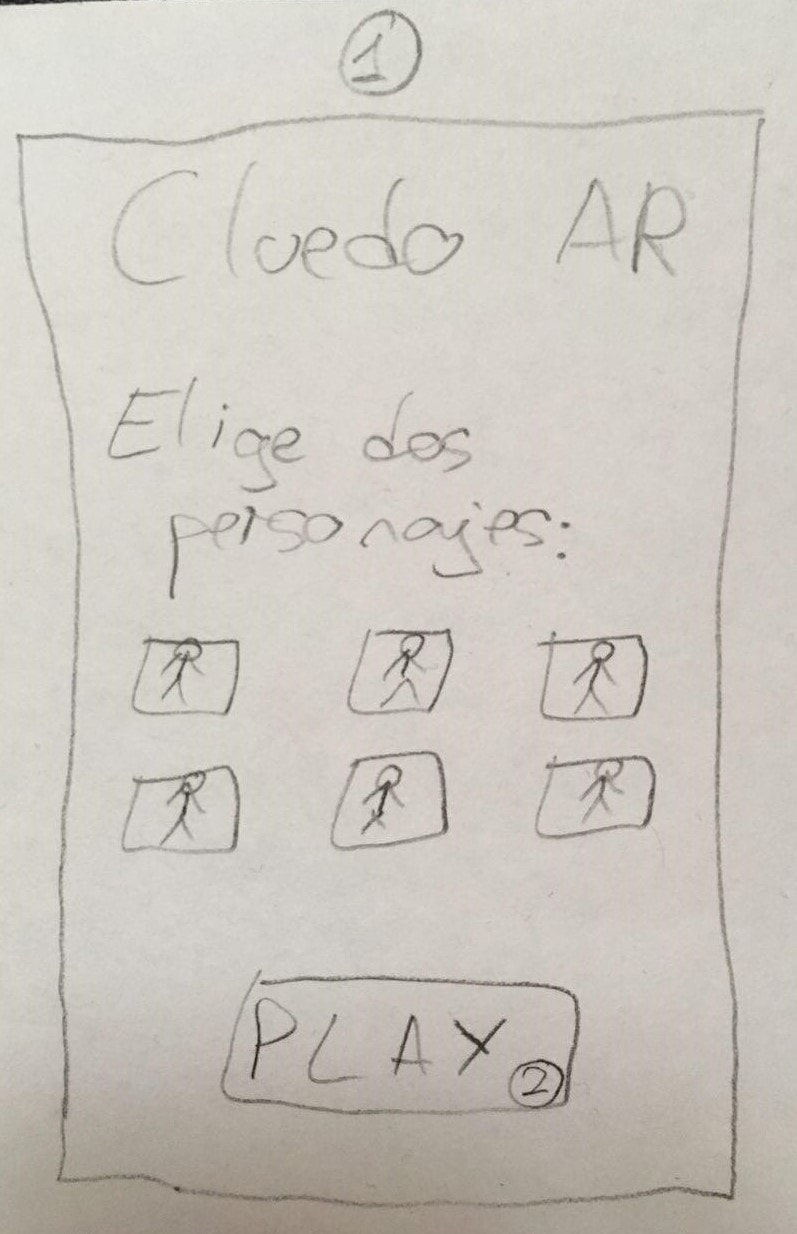
\includegraphics[height=2.48in]{b1.jpg}}
  \qquad
  \subfigure{
  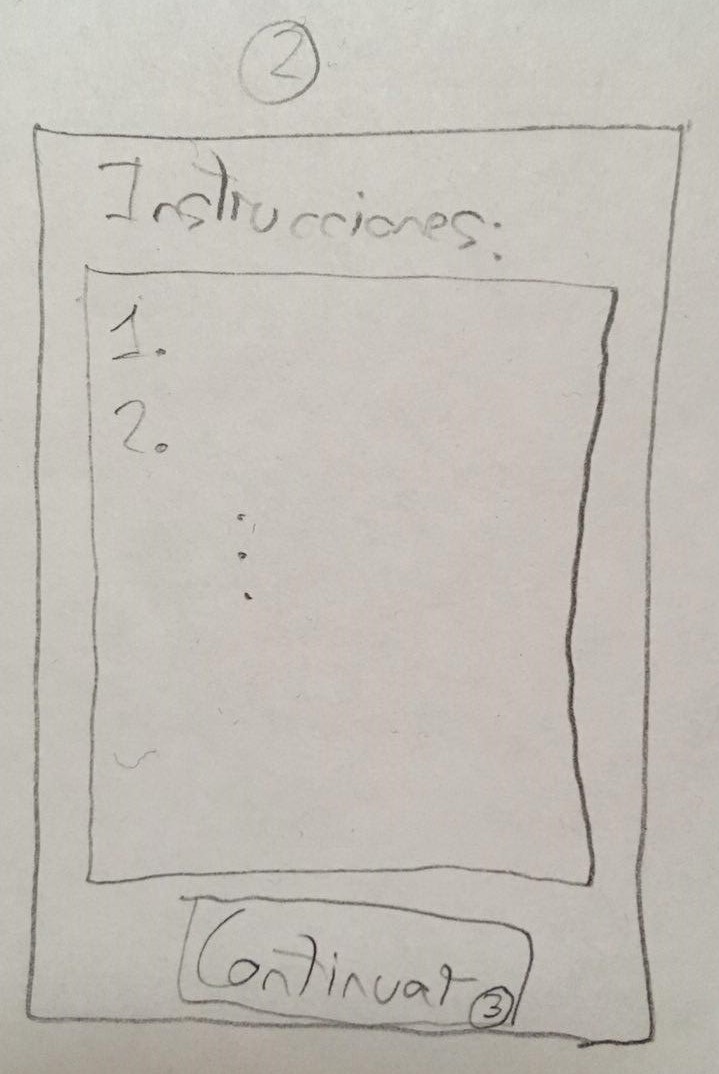
\includegraphics[height=2.48in]{b2.jpg}}
  \caption{Imagen que muestra los bocetos correspondientes a la interfaz inicial y la interfaz de instrucciones.}
\end{figure}

\begin{figure}[h]
  \subfigure{
  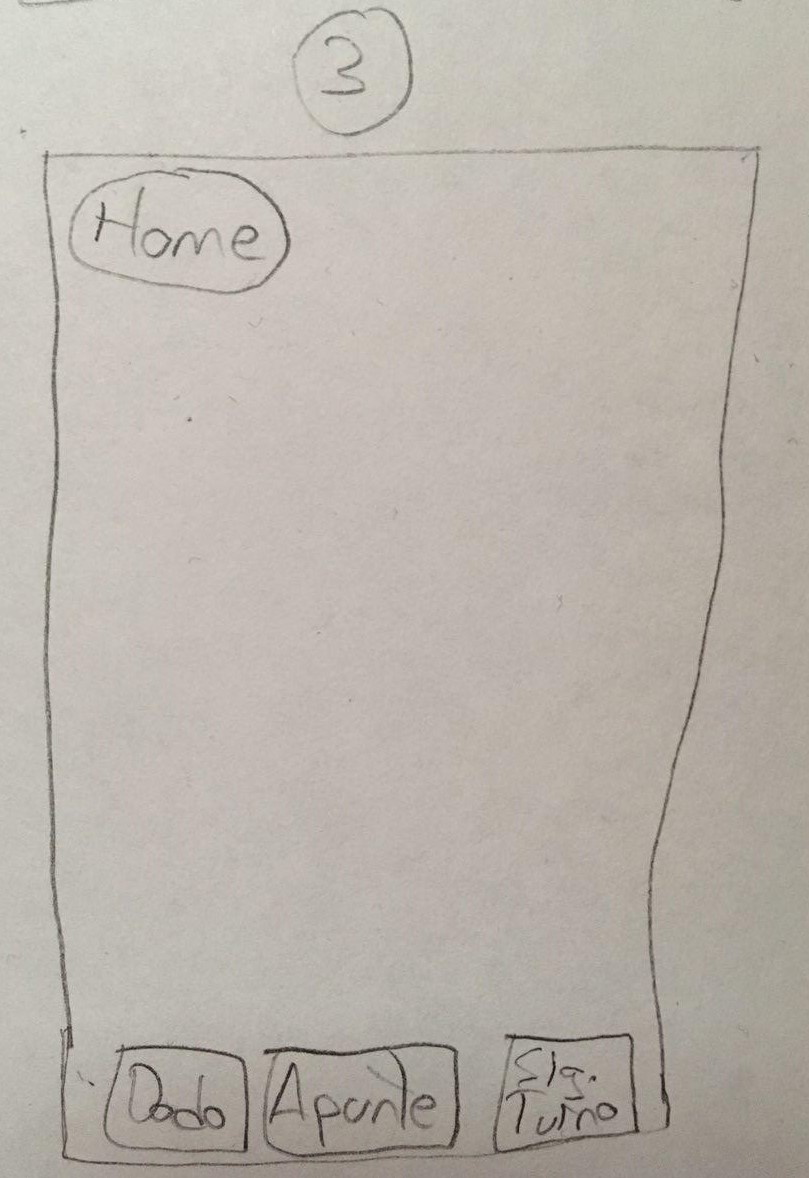
\includegraphics[height=2.47in]{b3.jpg}}
  \qquad
  \subfigure{
  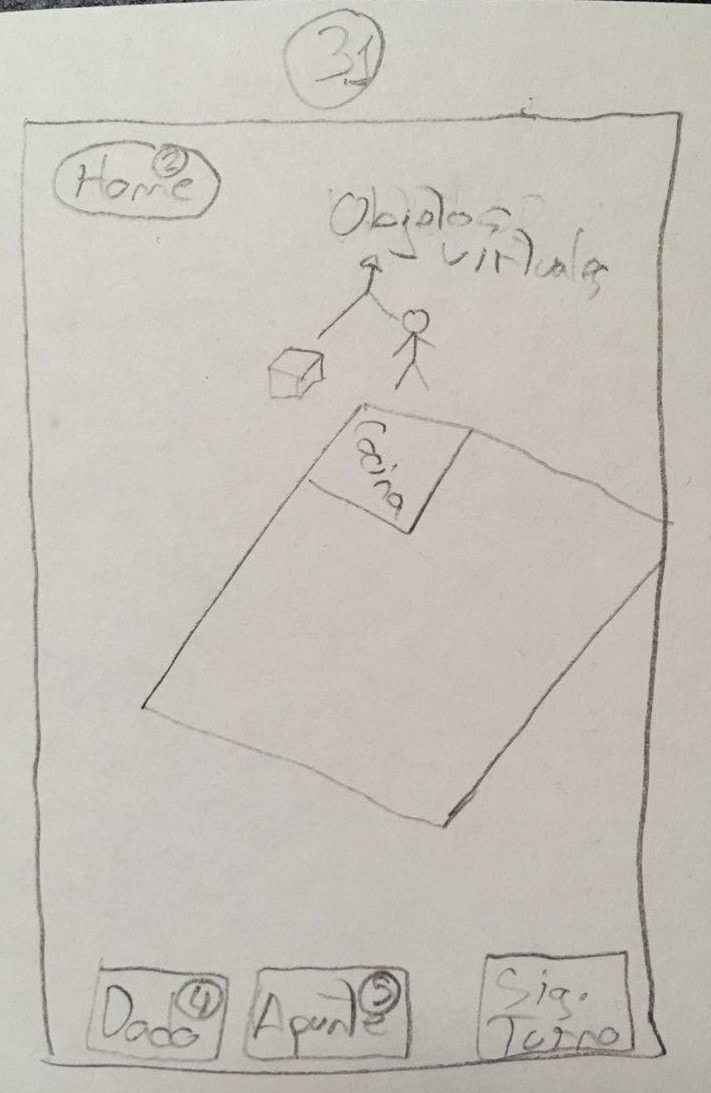
\includegraphics[height=2.52in]{b3-1.jpg}}
  \caption{Imagen que muestra los bocetos correspondientes a la interfaz de juego, en la derecha se esta escaneando el tablero.}
\end{figure}

\begin{figure}[h]
  \centering
  \subfigure{
  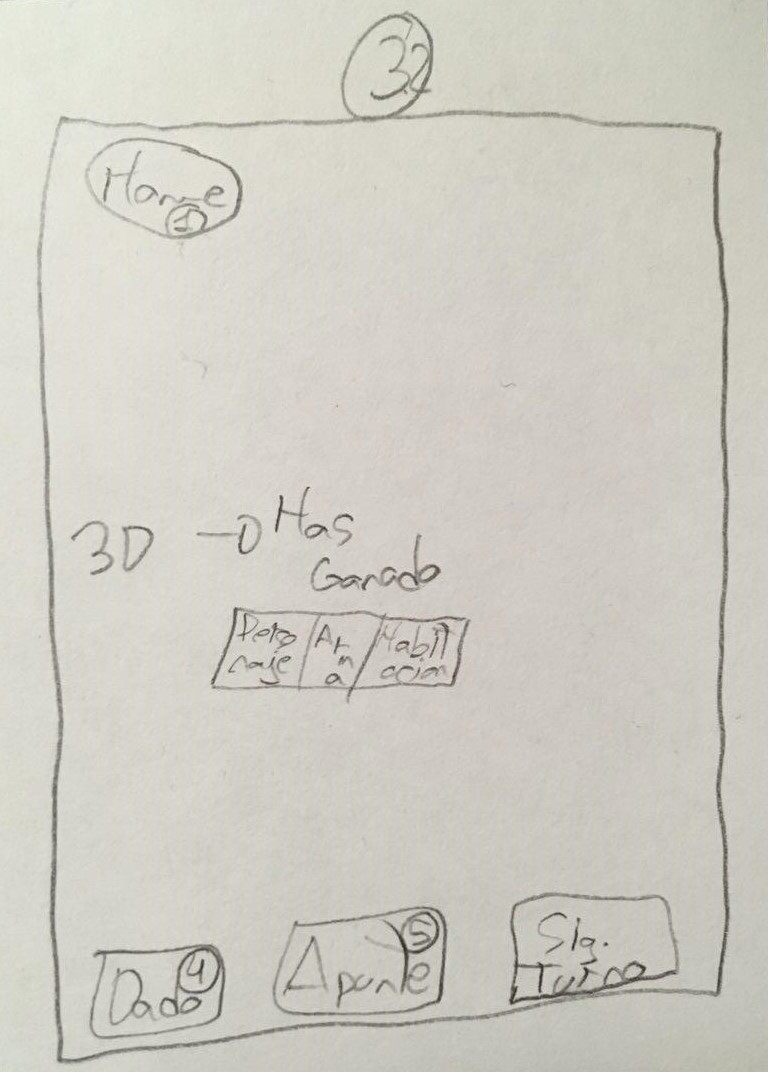
\includegraphics[height=2.5in]{b3-2.jpg}}
  \qquad
  \subfigure{
  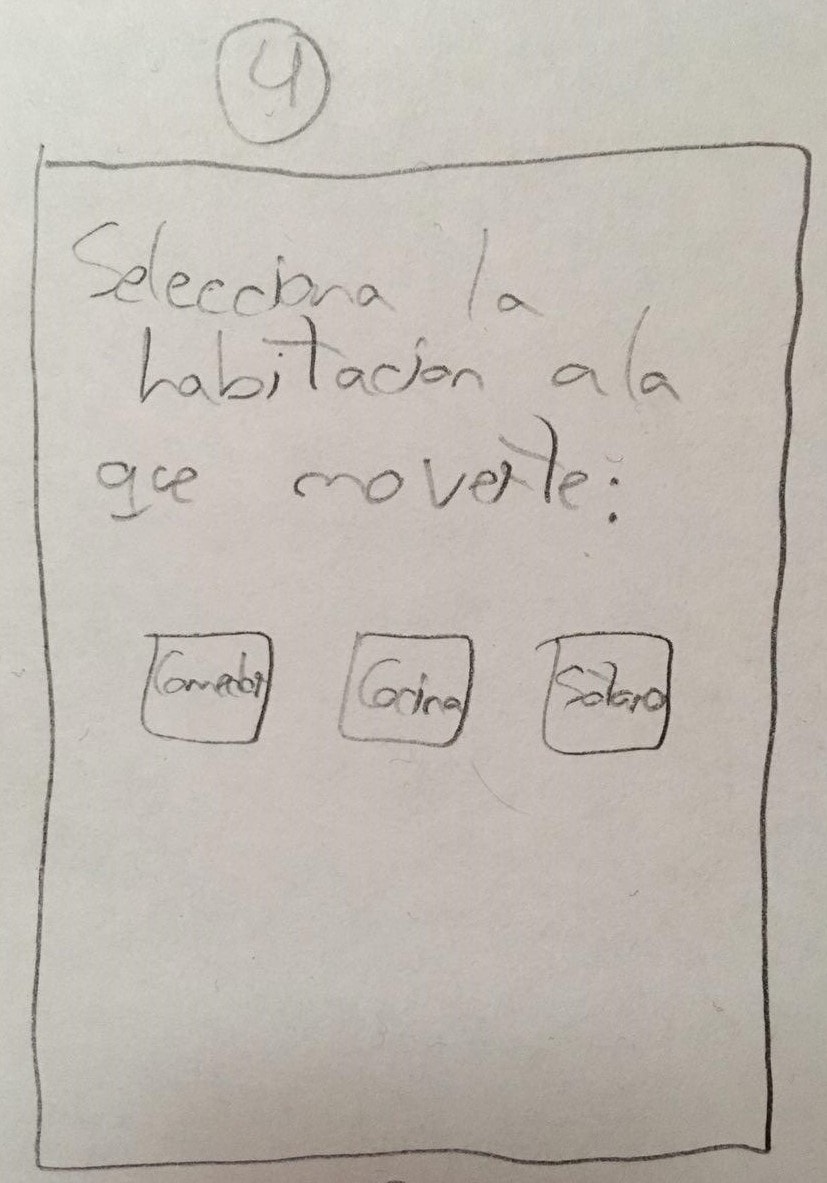
\includegraphics[height=2.5in]{b4.jpg}}
  \caption{Imagen que muestra los bocetos correspondientes a la interfaz de juego cuando se escanea una acusación, y a la interfaz de la seleción de habitación a la que moverse.}
\end{figure}

\begin{figure}[h]
  \centering
  \subfigure{
  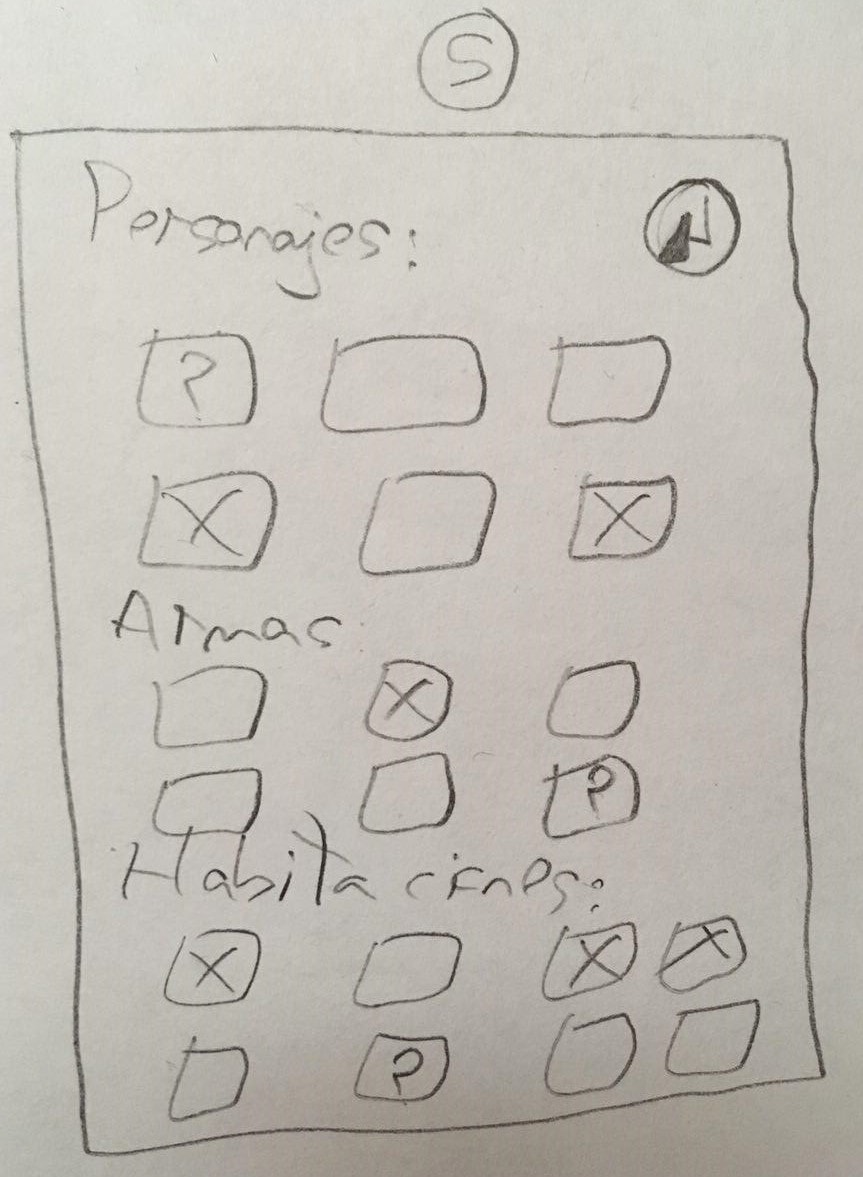
\includegraphics[height=2.5in]{b5.jpg}}
  \qquad
  \subfigure{
  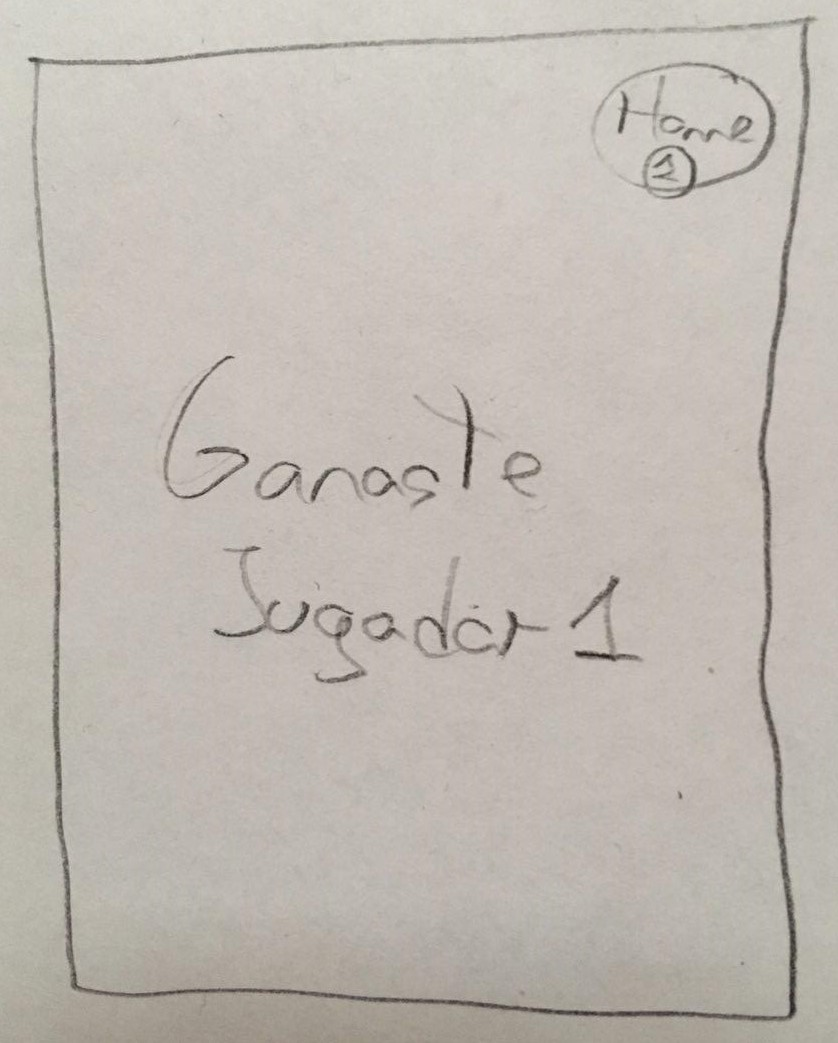
\includegraphics[height=2.5in]{b6.jpg}}
  \caption{Imagen que muestra los bocetos correspondientes a la interfaz de la toma de apuntes y la que indica que se ha ganado el juego.}
\end{figure}

\FloatBarrier

%%%%%%%%%%%%%%%%%%%%%%%%%%%%%%%%%%%%%%%%%%%%%%%%%%%%%% TABLAS USABILIDAD %%%%%%%%%%%%%%%%%%%%%%%%%%%%%%%%%%%%%%%%%%%%%%%%%%%%%%

\section{Tablas de usabilidad para los bocetos} \label{tablas-usabilidad-bocetos}

\begin{table}
  \begin{center}
    \begin{tabular}{|p{2.5cm}|p{1.75cm}|p{1.25cm}|p{1.25cm}|p{2.75cm}|p{3.5cm}|}

      \hline
        \rowcolor{Gray} \textbf{Escenario de uso}
        & \textbf{Tarea}
        & \textbf{Éxito/ Fracaso}
        & \textbf{Tiempo}
        & \textbf{Dificultades encontradas}
        & \textbf{Comentarios}\\

      \hline
      El usuario se encuentra jugando una partida
      & Seleccionar ajustes iniciales
      & Éxito
      & 10 seg
      & Le cuesta seleccionar el personaje con el dedo
      & Hacer los botones de personaje mas grandes para facilitar a los usuarios este proceso\\

      \hline
      El usuario se encuentra jugando una partida
      & Comenzar el juego
      & Éxito
      & 5 seg
      & Ninguna
      &\\

      \hline
      El usuario se encuentra jugando una partida
      & Salir de las instrucciones
      & Éxito
      & 5 seg
      & Ninguna
      &\\

      \hline
      El usuario se encuentra jugando una partida
      & Escanear el tablero
      & Éxito
      & 10 seg
      & Ninguna
      &\\

      \hline
      El usuario se encuentra jugando una partida
      & Lanzar el dado
      & Éxito
      & 20 seg
      & Ninguna
      & Añadir imagen con el nombre de la habitación para facilitar a los usuarios este proceso\\

      \hline
      El usuario se encuentra jugando una partida
      & Hacer apunte
      & Éxito
      & 25 seg
      & Ninguna
      &\\

      \hline
      El usuario se encuentra jugando una partida
      & Escanear acusación
      & Éxito
      & 20 seg
      & Ninguna
      &\\

      \hline
      El usuario se encuentra jugando una partida
      & Pasar de turno
      & Éxito
      & 5 seg
      & Ninguna
      &\\

      \hline
      El usuario se encuentra jugando una partida
      & Volver a la pantalla inicial
      & Fracaso
      & 15 seg
      & No sabe donde seleccionar terminar partida
      & Cambiar el texto del botón home por Terminar partida\\

      \hline
      El usuario se encuentra jugando una partida
      & Finalizar después de ganar
      & Éxito
      & 5 seg
      & No sabe donde seleccionar para salir de esa pantalla
      & Cambiar el texto del botón home por Continuar\\

      \hline

    \end{tabular}

    \caption{Resultados usabilidad con Usuario 1.}
    \label{tabla-bocetos-usuario1}

  \end{center}
\end{table}


\begin{table}
  \begin{center}
    \begin{tabular}{|p{2.5cm}|p{1.75cm}|p{1.25cm}|p{1.25cm}|p{2.75cm}|p{3.5cm}|}

      \hline
        \rowcolor{Gray} \textbf{Escenario de uso}
        & \textbf{Tarea}
        & \textbf{Éxito/ Fracaso}
        & \textbf{Tiempo}
        & \textbf{Dificultades encontradas}
        & \textbf{Comentarios}\\

      \hline
      El usuario se encuentra jugando una partida
      & Seleccionar ajustes iniciales
      & Éxito
      & 5 seg
      & Ninguna
      &\\

      \hline
      El usuario se encuentra jugando una partida
      & Comenzar el juego
      & Éxito
      & 5 seg
      & Ninguna
      &\\

      \hline
      El usuario se encuentra jugando una partida
      & Salir de las instrucciones
      & Éxito
      & 5 seg
      & Ninguna
      &\\

      \hline
      El usuario se encuentra jugando una partida
      & Escanear el tablero
      & Éxito
      & 15 seg
      & Ninguna
      &\\

      \hline
      El usuario se encuentra jugando una partida
      & Lanzar el dado
      & Éxito
      & 10 seg
      & Ninguna
      & \\

      \hline
      El usuario se encuentra jugando una partida
      & Hacer apunte
      & Fracaso
      & 25 seg
      & No comprendía el funcionamiento de cómo realizar un apunte
      & Explicar en la pantalla de instrucciones inicial como se realiza un apunte\\

      \hline
      El usuario se encuentra jugando una partida
      & Escanear acusación
      & Éxito
      & 10 seg
      & Ninguna
      &\\

      \hline
      El usuario se encuentra jugando una partida
      & Pasar de turno
      & Éxito
      & 3 seg
      & Ninguna
      &\\

      \hline
      El usuario se encuentra jugando una partida
      & Volver a la pantalla inicial
      & Fracaso
      & 7 seg
      & No encontraba el botón de inicio
      & Cambiar el texto del botón a español y mas grande\\

      \hline
      El usuario se encuentra jugando una partida
      & Finalizar después de ganar
      & Éxito
      & 3 seg
      & No sabe que significa home, el botón es pequeño y poco accesible
      & Cambiar el texto del botón a español y mas grande\\

      \hline

    \end{tabular}

    \caption{Resultados usabilidad con Usuario 2.}
    \label{tabla-bocetos-usuario2}

  \end{center}
\end{table}


\begin{table}
  \begin{center}
    \begin{tabular}{|p{2.5cm}|p{1.75cm}|p{1.25cm}|p{1.25cm}|p{2.75cm}|p{3.5cm}|}

      \hline
        \rowcolor{Gray} \textbf{Escenario de uso}
        & \textbf{Tarea}
        & \textbf{Éxito/ Fracaso}
        & \textbf{Tiempo}
        & \textbf{Dificultades encontradas}
        & \textbf{Comentarios}\\

      \hline
      El usuario se encuentra jugando una partida
      & Seleccionar ajustes iniciales
      & Éxito
      & 5 seg
      & Ninguna
      & Activar el botón de play cuando haya seleccionado 2 personajes\\

      \hline
      El usuario se encuentra jugando una partida
      & Comenzar el juego
      & Éxito
      & 5 seg
      & Ninguna
      &\\

      \hline
      El usuario se encuentra jugando una partida
      & Salir de las instrucciones
      & Éxito
      & 5 seg
      & Ninguna
      &\\

      \hline
      El usuario se encuentra jugando una partida
      & Escanear el tablero
      & Éxito
      & 3 seg
      & Ninguna
      &\\

      \hline
      El usuario se encuentra jugando una partida
      & Lanzar el dado
      & Éxito
      & 15 seg
      & El botón de dado no era muy descriptivo y el usuario no sabia si ahí se lanzaba
      & Cambiar el texto del botón dado a Lanzar dado\\

      \hline
      El usuario se encuentra jugando una partida
      & Hacer apunte
      & Éxito
      & 20 seg
      & El botón usuario no entiende que pasa al pulsar el botón de apunte
      & Cambiar el texto del botón de apunte a Notas\\

      \hline
      El usuario se encuentra jugando una partida
      & Escanear acusación
      & Éxito
      & 10 seg
      & Ninguna
      &\\

      \hline
      El usuario se encuentra jugando una partida
      & Pasar de turno
      & Éxito
      & 3 seg
      & Ninguna
      &\\

      \hline
      El usuario se encuentra jugando una partida
      & Volver a la pantalla inicial
      & Éxito
      & 3 seg
      & Ninguna
      &\\

      \hline
      El usuario se encuentra jugando una partida
      & Finalizar después de ganar
      & Éxito
      & 3 seg
      & Ninguna
      & Camiar el texto a Continuar y cambiar su posición y tamaño\\

      \hline

    \end{tabular}

    \caption{Resultados usabilidad con Usuario 3.}
    \label{tabla-bocetos-usuario3}

  \end{center}
\end{table}

\end{itemize}
